% easychair.tex,v 3.4 2015/12/10

\documentclass{easychair}
%\documentclass[EPiC]{easychair}
%\documentclass[debug]{easychair}
%\documentclass[verbose]{easychair}
%\documentclass[notimes]{easychair}
%\documentclass[withtimes]{easychair}
%\documentclass[a4paper]{easychair}
%\documentclass[letterpaper]{easychair}

\usepackage{doc}

% use this if you have a long article and want to create an index
% \usepackage{makeidx}

% In order to save space or manage large tables or figures in a
% landcape-like text, you can use the rotating and pdflscape
% packages. Uncomment the desired from the below.
%
% \usepackage{rotating}
% \usepackage{pdflscape}

% Some of our commands for this guide.
%
\newcommand{\easychair}{\textsf{easychair}}
\newcommand{\miktex}{MiK{\TeX}}
\newcommand{\texniccenter}{{\TeX}nicCenter}
\newcommand{\makefile}{\texttt{Makefile}}
\newcommand{\latexeditor}{LEd}

%\makeindex

%% Front Matter
%%
% Regular title as in the article class.
%
% \title{The {\easychair} Class File\\
%        Documentation and Guide for Authors%
% \thanks{Other people who contributed to this document include Maria Voronkov
%   (Imperial College and EasyChair) and Graham Gough (The University of
%   Manchester).}}

\title{Reconciling SCXML and Event-B Semantics}

% Authors are joined by \and. Their affiliations are given by \inst, which indexes
% into the list defined using \institute
%
% \author{
% Serguei A. Mokhov\inst{1}\thanks{Designed and implemented the class style}
% \and
%     Geoff Sutcliffe\inst{2}\thanks{Did numerous tests and provided a lot of suggestions}
% \and
%    Andrei Voronkov\inst{3}\inst{4}\inst{5}\thanks{Masterminded EasyChair and created versions
%      3.0--3.4 of the class style}
% }

\author{
Karla Morris\inst{1}
\and
Colin Snook\inst{2}
}

% Institutes for affiliations are also joined by \and,
\institute{
  Sandia National Laboratories, 
  Livermore, California, U.S.A.\\
  \email{knmorri@sandia.gov}
\and
   University of Southampton,
   Southampton, United Kingdom\\
   \email{cfs@ecs.soton.ac.uk}\\
 }

%  \authorrunning{} has to be set for the shorter version of the authors' names;
% otherwise a warning will be rendered in the running heads. When processed by
% EasyChair, this command is mandatory: a document without \authorrunning
% will be rejected by EasyChair

\authorrunning{}

% \titlerunning{} has to be set to either the main title or its shorter
% version for the running heads. When processed by
% EasyChair, this command is mandatory: a document without \titlerunning
% will be rejected by EasyChair

\titlerunning{}

\begin{document}

\maketitle

\begin{abstract}
  BLA BLA 
\end{abstract}

% The table of contents below is added for your convenience. Please do not use
% the table of contents if you are preparing your paper for publication in the
% EPiC series

\setcounter{tocdepth}{2}
{\small
\tableofcontents}

%\section{To mention}
%
%Processing in EasyChair - number of pages.
%
%Examples of how EasyChair processes papers. Caveats (replacement of EC
%class, errors).

\pagestyle{empty}

%------------------------------------------------------------------------------
\section{Introduction}
\label{sect:introduction}


% \begin{figure}[tb]
% 	\begin{centering}
% 	
\includegraphics[width=0.5\textwidth]{logoEC}
% 	\caption{EasyChair logo}
% 	\label{fig:easychair-logo}
% 	\end{centering}
% \end{figure}

This section should focus on the motivation behind pursuing a scxml 
representation of our models, what are the benefits?

%------------------------------------------------------------------------------

\section{Differences in Semantics}
\label{sect:diff}

Differences in semantics between scxml and event-b

Elude to the reason for ignoring some of the scxml feature 
when it comes to the translation.

List the difference in the syntax of each representation (Short section)

%------------------------------------------------------------------------------

\section{Reconciling Semantics}
\label{sect:recon}

Reconciling scxml semantics for event-b code generation.  
(Important, people will be interested

%------------------------------------------------------------------------------

\section{Extending SCXML}
\label{sect:extension}

Methodology for adding required information to allow refinement, invariants,
guards, variable type declaration.

%------------------------------------------------------------------------------

\section{Case Study}
\label{sect:caseS}

Find a system that we can model and some how describe the benefits 
(e.g. model simplification) of using a specific syntax over the other.
	\begin{itemize}
		\item What model behavior can you capture with each semantic?
		\item What properties of the model are easier to simulate?
		\item Where do we introduce unnecessary complexity?
	\end{itemize}	


%------------------------------------------------------------------------------
\section{Conclusion}
\label{sect:concl}

Just to have a reference ~\cite{texniccenter}

%------------------------------------------------------------------------------
\section{Future Work}
\label{sect:future-work}


% \begin{figure}[tb]
%   \begin{centering}
%     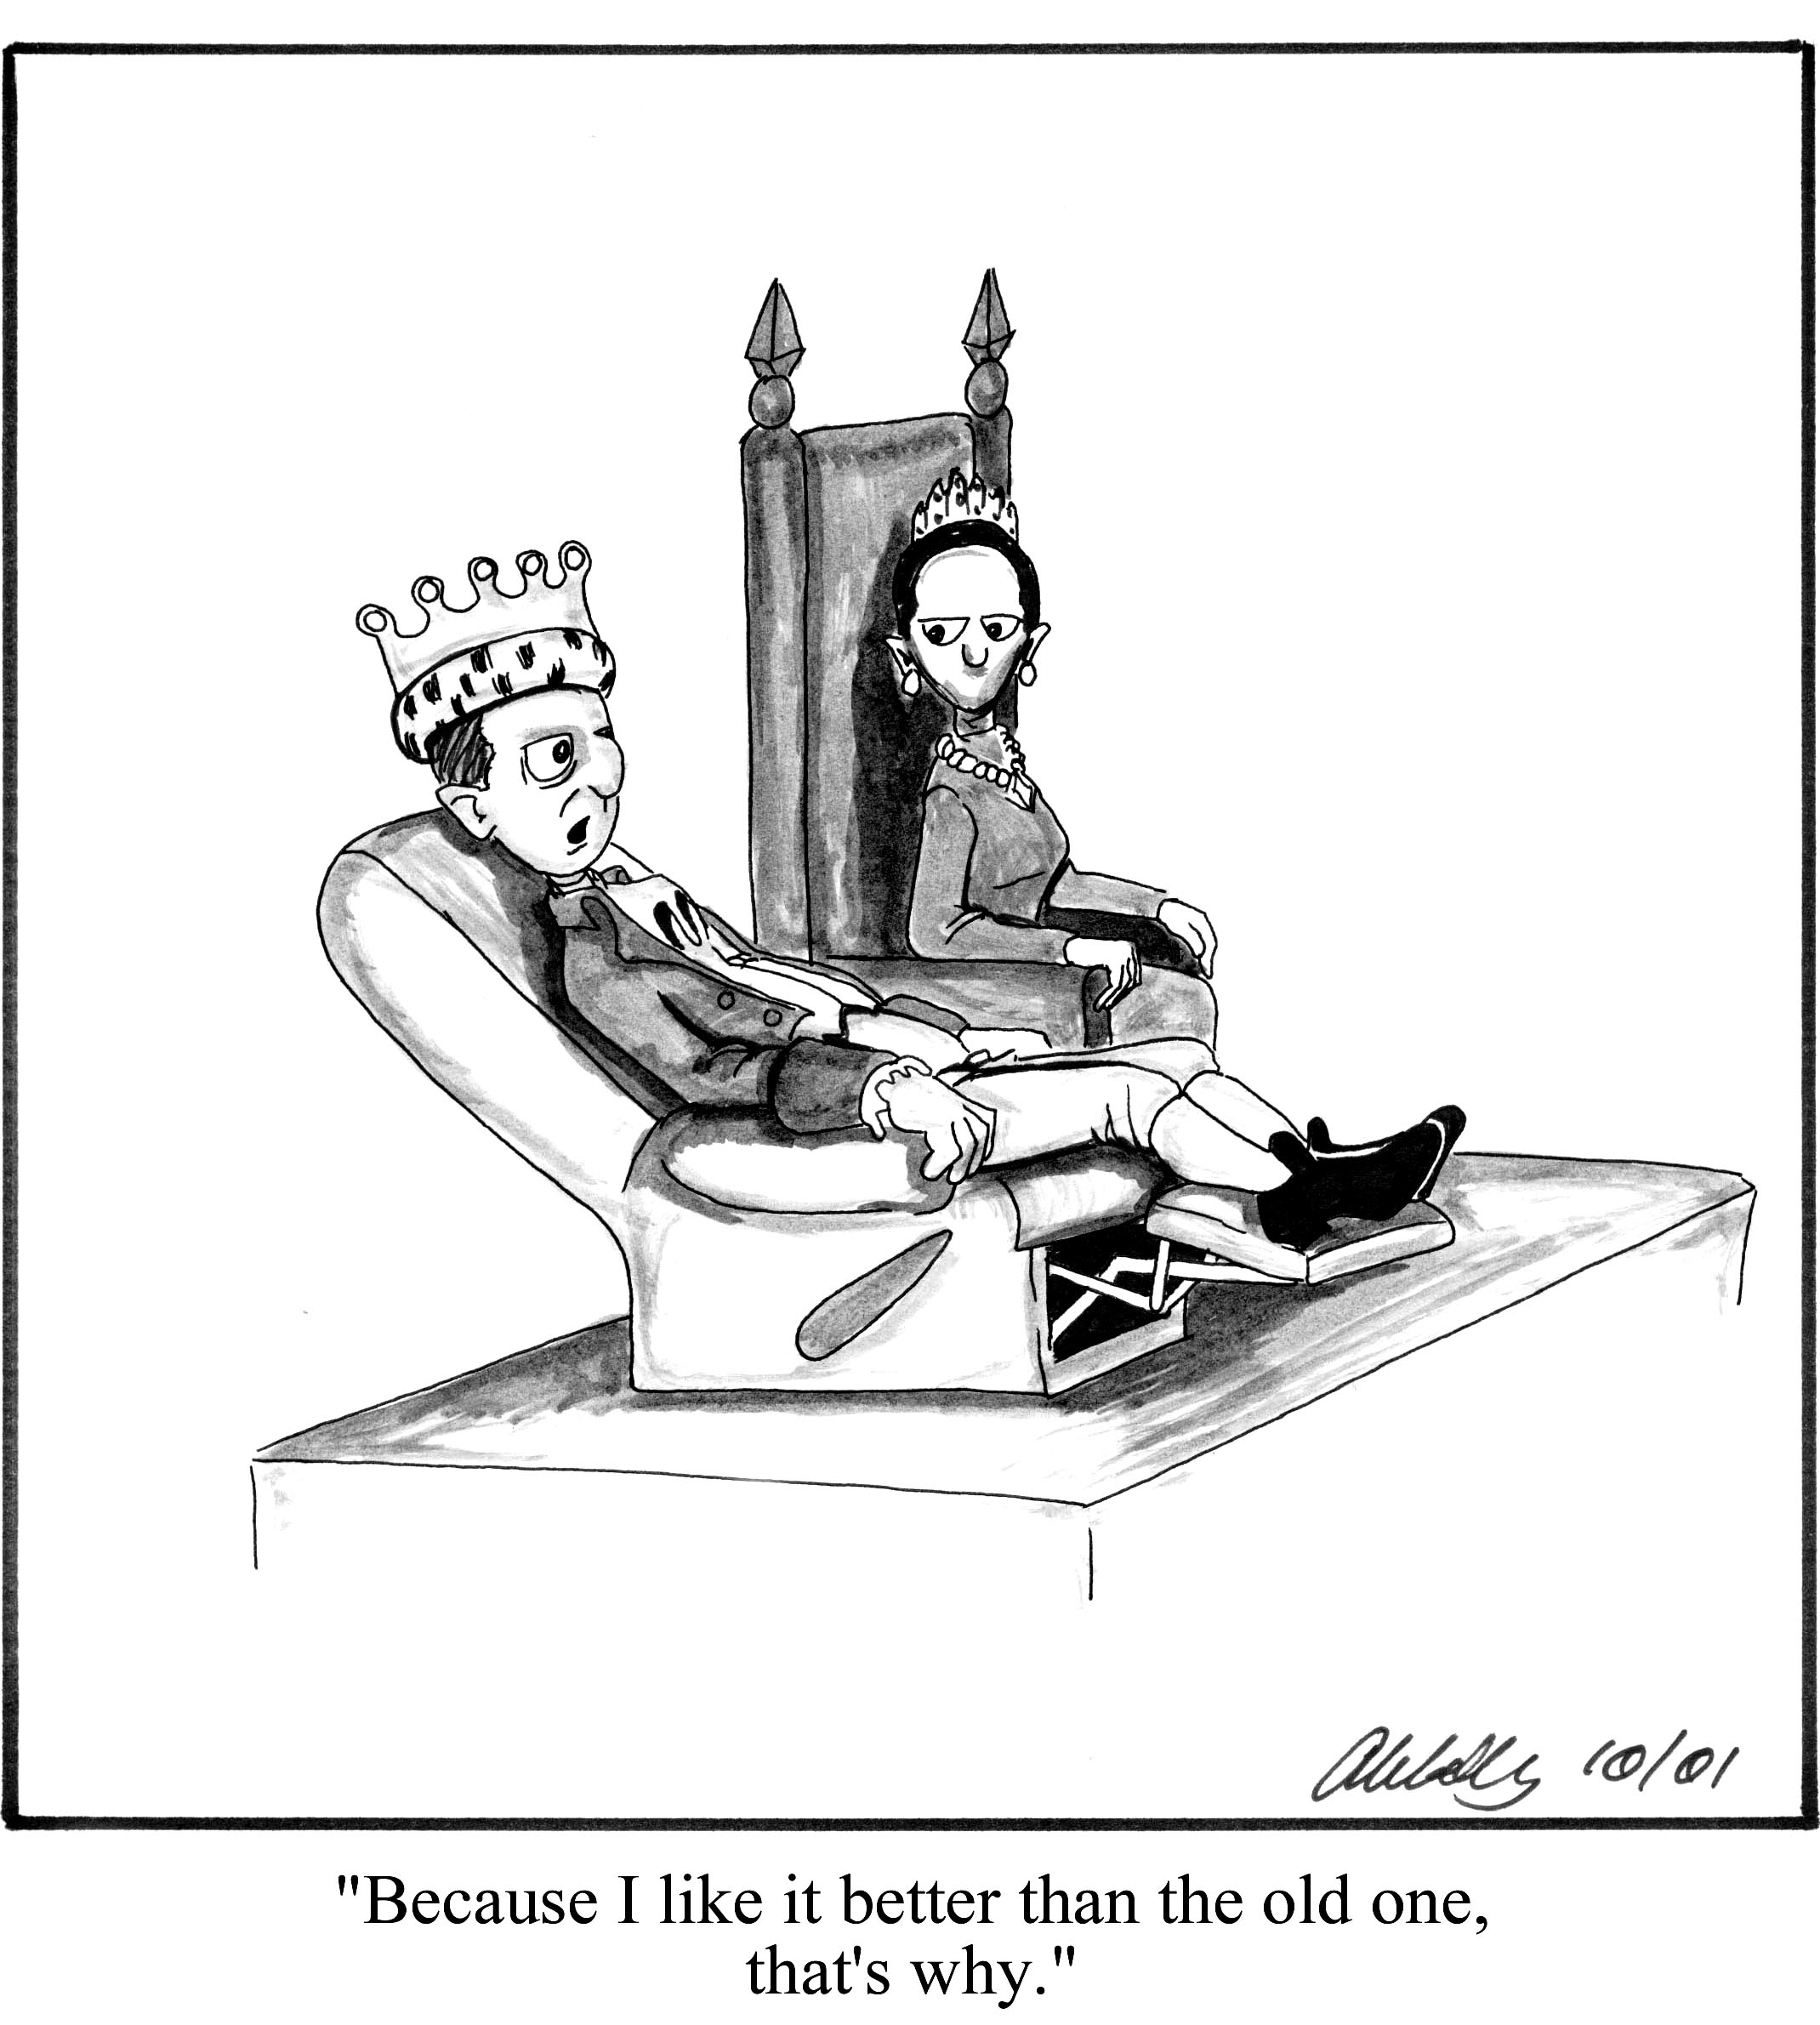
\includegraphics[width=0.5\textwidth]{throneEC.jpg}
%     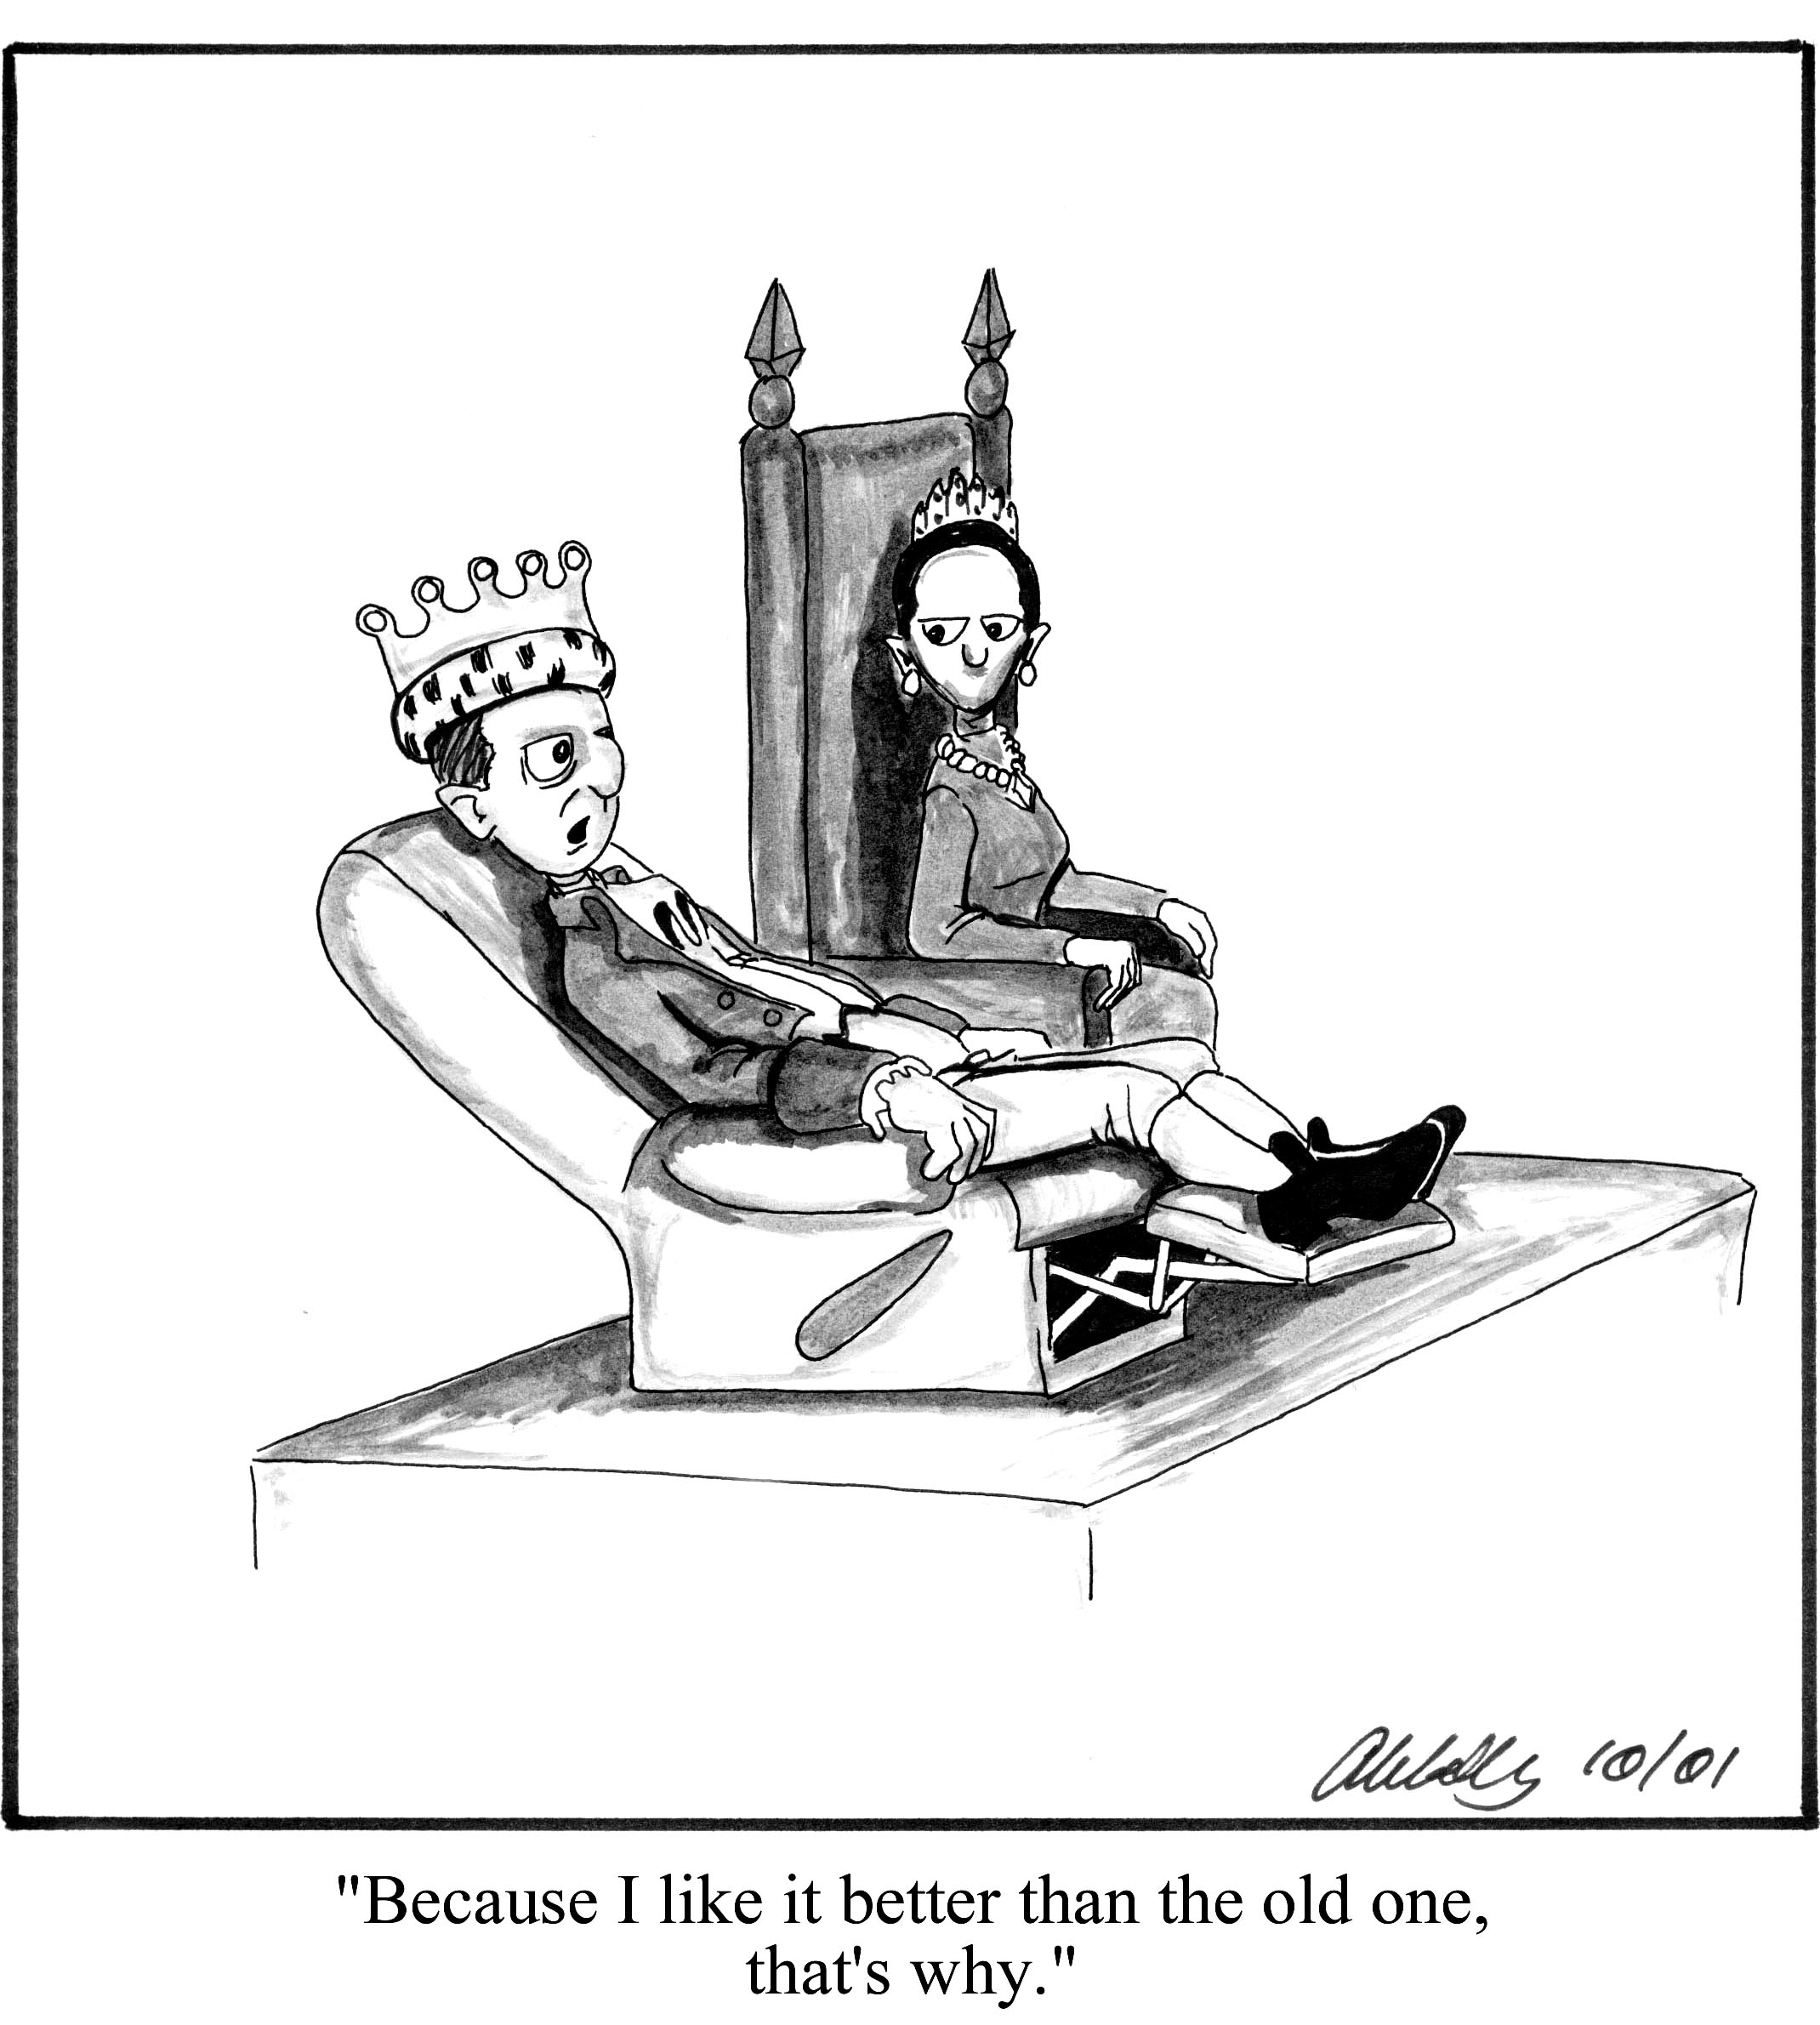
\includegraphics[width=0.3\textwidth]{throneEC.jpg}
%     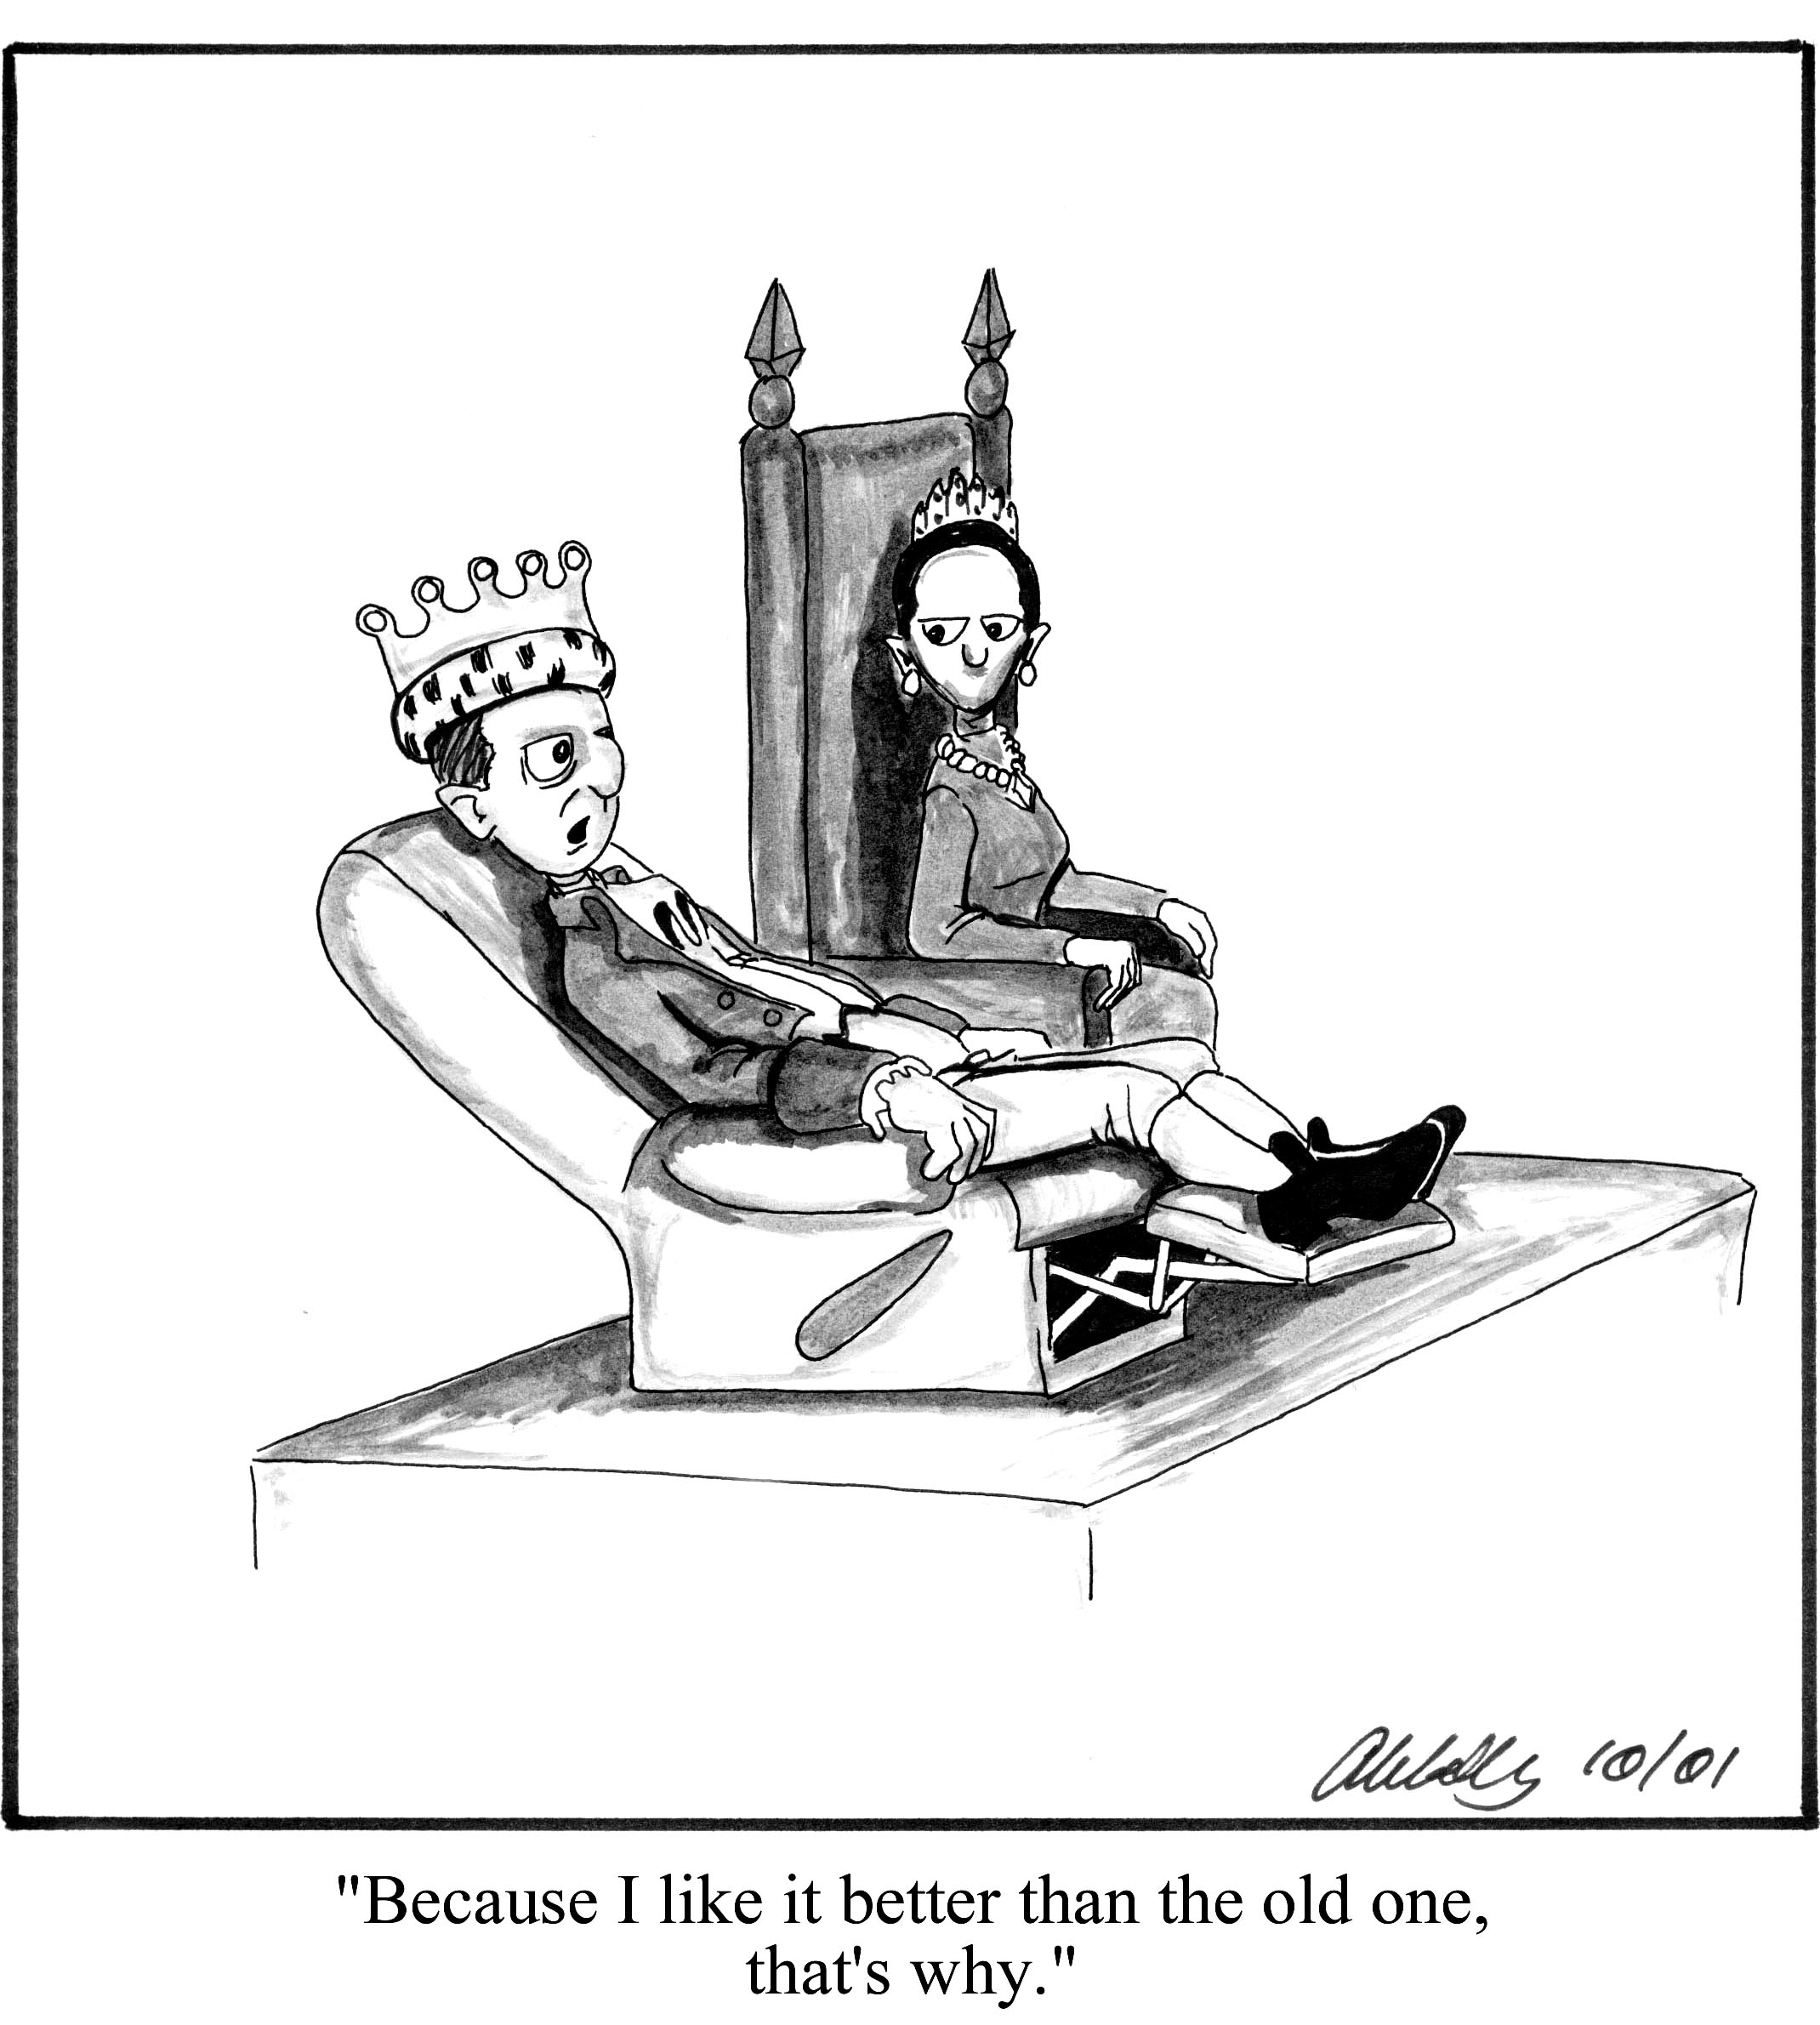
\includegraphics[width=0.15\textwidth]{throneEC.jpg}
%   \end{centering}
%   \caption{Why one should use EasyChair}
%   \label{fig:easythrone}
% \end{figure}

%------------------------------------------------------------------------------
\section{Acknowledgments}
\label{sect:acks}


\label{sect:bib}
\bibliographystyle{plain}
%\bibliographystyle{alpha}
%\bibliographystyle{unsrt}
%\bibliographystyle{abbrv}
\bibliography{easychair}

%------------------------------------------------------------------------------

%------------------------------------------------------------------------------
% Index
%\printindex

%------------------------------------------------------------------------------
\end{document}

